\chapter{Fields}
\label{chapter:Fields}
\thispagestyle{empty}


In Chapter~\ref{chapter:PolyEquations}, we explored problems about finding and expressing roots of polynomials, finally arriving at the goal of the course: proving that there are quintic polynomials that are \emph{not} solvable by radicals. This chapter serves two main purposes. First, as we look at roots of polynomials and how they can be expressed, it will be convenient to have a common world (i.e.~number system) in which they live. For us, this will be the complex numbers, denoted $\mathbb{C}$, which will be reviewed below. Our work with complex numbers will also supply the necessary language to properly talk about $n^{\text{th}}$-roots. Second, we are still in need of a proper definition of what it means for a polynomial to be ``solvable by radicals''; this is where the chapter will finish. But the middle of the chapter is perhaps the most interesting. There, on the way to defining ``solvable by radicals'', we will be led to abstract the structure of $\mathbb{C}$ (and of $\mathbb{Q}$ and $\mathbb{R}$), arriving at the definition of a \emph{field}. 

% % % % % % % % % % % % % % % % % % % % % % % % % % % % % % % % % % % % % % % % % % % %
% % % % % % % % % % % % % % % % % % % % % % % % % % % % % % % % % % % % % % % % % % % %
% SECTION
% % % % % % % % % % % % % % % % % % % % % % % % % % % % % % % % % % % % % % % % % % % %
% % % % % % % % % % % % % % % % % % % % % % % % % % % % % % % % % % % % % % % % % % % %
\begin{section}{Complex Numbers}
As mentioned above, we want to work in a world that contains all of the roots of all of the polynomials that we will be studying. Considering the roots of polynomials such as $x^2 +1$, $x^2-2$, $x^2-3$, etc., we see that we need to include numbers like $\sqrt{-1}$, $\sqrt{2}$, $\sqrt{3}$, etc., so although there are smaller worlds one could choose, we will opt for the world containing both $\sqrt{-1}$ and $\mathbb{R}$, namely $\mathbb{C}$.

But before we proceed, note that $\sqrt{-1}$ is not really well defined. There are \emph{two} solutions to $x^2 +1$, so when we write $\sqrt{-1}$, we are all agreeing that we mean the same one. 

\begin{definition}
Let $i$ (or alternatively $\sqrt{-1}$) denote one particular solution to $x^2 +1$. 
\end{definition}

Of course, the previous definition implies that $i^2 = -1$. Using $i$ and $\mathbb{R}$, we now build the complex numbers.

% % % % % % % % % % % % % % % % % % % % % % % % % % % % % % % % % % % % % % % % % % % %
% SUBSECTION
% % % % % % % % % % % % % % % % % % % % % % % % % % % % % % % % % % % % % % % % % % % %
\subsection{Definition and first principles}

\begin{definition}
The \textbf{complex numbers} is the set $\mathbb{C} := \{a + bi\mid a,b \in \mathbb{R}\}$. If $z=a+bi$, then $a$ is called the \textbf{real part} of $z$ and $b$ is called the \textbf{imaginary part} of $z$.
\end{definition}

Note that every complex number $z=a+bi$ is uniquely determined by two numbers: the real and imaginary parts $a$ and $b$. As such, we often graph complex numbers in the coordinate plane with the $x$-axis denoting the real part and the $y$-axis denoting the imaginary part. This will be called the \textbf{complex plane}.

\begin{example}
We graph $-2 + 2i$ and  $1 - 3i$ below.
\begin{center}
\begin{tikzpicture}[line width = .9,scale = .7]
\draw[<->] (-4,0) -- (4,0) node [below] {\small \textsc{Real}};
\draw[<->] (0,-4) -- (0,4) node [left] {\small \textsc{Imag.}};
\foreach \i in {1,2,3} {
\draw (-\i,-0.1) -- (-\i,0.1);
\draw (\i,-0.1) -- (\i,0.1);
\node[anchor = 90] at (-\i,0) {\small $\i$};
\node[anchor = 90] at (\i,0) {\small $\i$};
\draw (-0.1,-\i) -- (0.1,-\i);
\draw (-0.1,\i) -- (0.1,\i);
\node[anchor = 0] at (0,-\i) {\small $\i$};
\node[anchor = 0] at (0,\i) {\small $\i$};
}
\node (w) at (-2,2) {};
\fill (w) circle (.1);
\node[anchor = -10] at (w) {\small $-2 + 2i$};
\node (z) at (1,-3) {};
\fill (z) circle (.1);
\node[anchor = 170] at (z) {\small $1 - 3i$};
\end{tikzpicture}
\end{center}
\end{example}

We also define some operations on complex numbers.

\begin{definition}
We define the following operations on elements of $\mathbb{C}$. 
\begin{itemize}
\item \textbf{Addition:} $(a+bi) + (c+di) := (a+b) + (c+d)i$
\item \textbf{Multiplication:} $(a+bi) \cdot (c+di) := (ac-bd) + (ad+bc)i$
\item \textbf{Complex Conjugation:} $\overline{a+bi} := a-bi$
\end{itemize}
\end{definition}

Notice that in the definition of complex multiplication we are just using the normal distributive law (or FOIL if you like) together with the fact that $i^2 = -1$. Many of the familiar algebraic properties of $\mathbb{R}$ also hold for $\mathbb{C}$, which we will take as a fact.

\begin{fact}\label{fact.ComplexLaws} The following are true for $\mathbb{C}$.
\begin{itemize}
\item \textbf{Addition Laws:} Addition is associative and commutative. There is a unique additive identity, namely $0 = 0 + 0i$, and every number has a unique additive inverse, denoted $-(a+bi)$.
\item \textbf{Multiplication Laws:} Multiplication is associative and commutative. There is a unique multiplicative identity, namely $1 = 1 + 0i$, and every nonzero number has a unique multiplicative inverse, denote $(a+bi)^{-1}$ or $\frac{1}{a+bi}$.
\item \textbf{Distributivity Laws:} For all $x,y,z \in \mathbb{C}$, $x(y+z) = xy+xz$ and $(y+z)x = yx+zx$.
\item \textbf{Conjugation Laws:} For all $x,y \in \mathbb{C}$, $\overline{x+y} = \overline{x} + \overline{y}$ and $\overline{xy} = \overline{x}\overline{y}$.
\end{itemize}
\end{fact}

\begin{problem}
Thinking of a complex number $z=a+bi$ as a point in the complex plane, describe \emph{geometrically} what happens when $(c+di)$ is added to $z$. Also, describe \emph{geometrically}  how to find $\overline{z}$ from $z$.
\end{problem}

When we plot points, there are different coordinate systems we could use. It turns out that  rectangular coordinates are good for adding complex numbers, but polar coordinates are better for multiplication. This lead to the following definition.

\begin{definition}
Let $z=a+bi$. 
\begin{enumerate}
\item The \textbf{modulus} of $z$, denoted $|z|$, is the radius of the point $(a,b)$ when written in polar coordinates. Thus, $|z| = \sqrt{a^2 + b^2}$. 
\item The \textbf{argument} of $z$, denoted $\Arg(z)$, is the angle of the point $(a,b)$ when written in polar coordinates. Thus, $\Arg(z)$ is the angle $\theta$ \emph{in the appropriate quadrant} such that $0\le \theta<2\pi$ and $\tan \theta = \frac{b}{a}$. The argument of  $0$ is undefined.
\end{enumerate}
\end{definition}

\begin{example}
We have that $|-2 + 2i| = \sqrt{(-2)^2+2^2} = 2\sqrt{2}$ and $\Arg(-2 + 2i) = \frac{3\pi}{4}$. (But be careful, $\arctan\left(\frac{2}{-2}\right) = \frac{\pi}{4}$; you must pay attention to which quadrant the number is in.)
\begin{center}
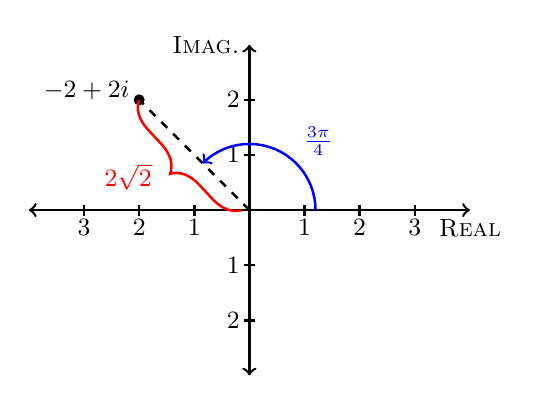
\begin{tikzpicture}[line width = .9,scale = .7]
\small
\draw[<->] (-4,0) -- (4,0) node [below] { \textsc{Real}};
\draw[<->] (0,-3) -- (0,3) node [left] { \textsc{Imag.}};
\foreach \i in {1,2,3} {
\draw (-\i,-0.1) -- (-\i,0.1);
\draw (\i,-0.1) -- (\i,0.1);
\node[anchor = 90] at (-\i,0) { $\i$};
\node[anchor = 90] at (\i,0) { $\i$};
}
\foreach \i in {1,2} {
\draw (-0.1,-\i) -- (0.1,-\i);
\draw (-0.1,\i) -- (0.1,\i);
\node[anchor = 0] at (0,-\i) { $\i$};
\node[anchor = 0] at (0,\i) { $\i$};
}
\node (w) at (-2,2) {};
\fill (w) circle (.1);
\node[anchor = -10] at (w) { $-2 + 2i$};

\draw [dashed] (0,0) -- (w.center);
\draw [blue,domain=0:135,->] plot ({1.2*cos(\x)}, {1.2*sin(\x)});
\node[blue] at (1.25,1.25) {$\frac{3\pi}{4}$};

\draw [red,decorate,decoration={brace,amplitude=10pt},xshift=-4pt,yshift=0pt]
(0,0) -- (w.center);
\node[red] at (-2.2,0.6) {$2\sqrt{2}$}; 
\end{tikzpicture}
\end{center}
\end{example}

\begin{problem}\label{prob.ComplexCheckin}
For each of the following complex numbers,
\begin{itemize}
\item write it in the form $a+bi$ (if it is not already),
\item plot it in the complex plane,
\item find the modulus and argument (if not exact, then a decimal approximation is okay).
\end{itemize}
\begin{multicols}{2}
\begin{enumerate}
\item $u = -1-i$
\item $v= \frac{1}{1+i}$
\item $w = \frac{(2-i)(1+2i)}{2+3i}$
\item $z\in \mathbb{C}$ with $|z| = 3$ and $\Arg(z) = \frac{4\pi}{3}$
\end{enumerate}
\end{multicols}
\end{problem}

\begin{theorem}
Let $z\in \mathbb{C}$. If $z\neq 0$, then $z^{-1} = \displaystyle\frac{\overline{z}}{|z|^2}$.
\end{theorem}

The next theorem shows how to find an expression for a complex number given its modulus and argument.
 
\begin{theorem}\label{thm.PolarToRectangular}
Let $z\in \mathbb{C}$. Then $|z| = r$ and $\Arg(z) = \theta$ if and only if $z = r\cos\theta + ir\sin\theta$ with $0\le \theta <2\pi$.
\end{theorem}

We now derive some properties of multiplication. The first is quite useful and illustrates how multiplication is rather easy to deal with when numbers are in ``polar form''.

\begin{theorem}\label{thm.MultiplyComplex}
If $z_1 = r_1\cos\theta_1 + ir_1\sin\theta_1$ and $z_2=r_2\cos\theta_2 + ir_2\sin\theta_2$, then \[z_1z_2 = r_1r_2\cos(\theta_1+\theta_2) + ir_1r_2\sin(\theta_1+\theta_2).\]
\end{theorem}

\begin{corollary}
If $z_1,z_2\in \mathbb{C}$, then $|z_1z_2| = |z_1||z_2|$ and $\Arg(z_1z_2) = \Arg(z_1)+\Arg(z_2)$.
\end{corollary}

\begin{corollary}[De Moivre's formula]\label{cor.DeMoivre}
For each positive $n\in \mathbb{Z}$, \[\left(r\cos(\theta) + ir\sin(\theta)\right)^n = r^n\cos(n\theta) + ir^n\sin(n\theta).\]
\end{corollary}

% % % % % % % % % % % % % % % % % % % % % % % % % % % % % % % % % % % % % % % % % % % %
% SUBSECTION
% % % % % % % % % % % % % % % % % % % % % % % % % % % % % % % % % % % % % % % % % % % %
\subsection{Roots of unity}
We now arrive at an \emph{extremely important} definition.

\begin{definition}
For each positive $n\in \mathbb{Z}$, define \[\zeta_n := \cos\left(\frac{2\pi}{n}\right) + i\sin\left(\frac{2\pi}{n}\right).\]
Thus, $\zeta_n$ (read as ``zeta n'') is the unique  number with magnitude $1$ and argument $\frac{2\pi}{n}$.
\end{definition}

\begin{problem}
Plot each of the following in the same complex plane: $\zeta_2$, $\zeta_3$, $\zeta_4$, $\zeta_5$.
\end{problem}

\begin{problem}
Plot each of the following in the same complex plane: $\zeta_6$, $(\zeta_6)^2$, $(\zeta_6)^3$, $(\zeta_6)^4$, $(\zeta_6)^5$, $(\zeta_6)^6$.
\end{problem}

\begin{problem}
Write $\overline{\zeta_8}$ as a power of $\zeta_8$. Conjecture and prove a formula that expresses $\overline{(\zeta_n)^k}$ as a power of $\zeta_n$, but with no bar on top.
\end{problem}

We now turn our attention back to solving polynomial equations, focusing on those of the form $x^n - a$.

\begin{definition}
Let $a\in \mathbb{C}$. A number $z\in \mathbb{C}$ is called an \textbf{$n^\text{th}$ root of $a$} if $z^n = a$. In other words, the  $n^\text{th}$ roots of $a$ are the roots of the polynomial $x^n-a$. The  $n^\text{th}$ roots of $1$ are also called \textbf{$n^\text{th}$ roots of unity}.
\end{definition}

\begin{problem}
Find a $4^\text{th}$ root of each of the following: $\zeta_3$ and $-1 + i\sqrt{3}$.
\end{problem}

\begin{theorem}
For each non-negative $k\in \mathbb{Z}$, $(\zeta_n)^k$ is an $n^\text{th}$ root of $1$.
\end{theorem}

\begin{lemma}\label{lem.nthRoot1IsPowerOfZeta}
If $z$ is an $n^\text{th}$ root of $1$, then $z = (\zeta_n)^k$ for some non-negative $k\in \mathbb{Z}$.
\end{lemma}

\begin{lemma}
For each non-negative $k\in \mathbb{Z}$, $(\zeta_n)^k = (\zeta_n)^m$ for some $0\le m \le n-1$.
\end{lemma}

\begin{theorem}\label{thm.nthRoots1}
The set \[\{1, \zeta_n, (\zeta_n)^2, \ldots, (\zeta_n)^{n-1}\}\] is the set of \emph{all} $n^\text{th}$ roots of unity. Thus, there are $n$ distinct $n^\text{th}$ roots of unity. 
\end{theorem}

\begin{lemma}
Let $a\in \mathbb{C}$ be nonzero, and let $b$ be any one particular $n^\text{th}$ root of $a$. Then $z$ is an $n^\text{th}$ root of $a$ if and only if $\frac{z}{b}$ is an $n^\text{th}$ root of $1$.
\end{lemma}

\begin{theorem}\label{thm.nthRoots}
Let $a\in \mathbb{C}$ be nonzero, and let $b$ be any one particular $n^\text{th}$ root of $a$. The set \[\{b, b\zeta_n, b(\zeta_n)^2, \ldots, b(\zeta_n)^{n-1}\}\] is the set of \emph{all} $n^\text{th}$ roots of $a$. Thus, there are $n$ distinct $n^\text{th}$ roots of $a$. 
\end{theorem}

\begin{problem}
Find \emph{all} $4^\text{th}$ roots of each of the following: $\zeta_3$ and $-1 + i\sqrt{3}$.
\end{problem}

% % % % % % % % % % % % % % % % % % % % % % % % % % % % % % % % % % % % % % % % % % % %
% SUBSECTION
% % % % % % % % % % % % % % % % % % % % % % % % % % % % % % % % % % % % % % % % % % % %
\subsection{Roots of polynomials over  $\mathbb{R}$ and  $\mathbb{C}$}
We conclude this section with a couple of general results about roots of polynomials.

\begin{theorem}\label{thm.RootsRealCoeff}
Suppose that $p(x) = a_nx^n + a_{n-1}x^{n-1} +\cdots+a_2x^2+a_1x+a_0$ with all $a_i\in \mathbb{R}$. If $z$ is a root of $p(x)$, then $\overline{z}$ is also a root of $p(x)$.
\end{theorem}

In words, the previous theorem says that if a polynomial has coefficients in $\mathbb{R}$, then the set of roots is ``closed under complex conjugation.'' We end with an extremely important theorem, which will be quite useful for us. However, since its proof is not our main goal (and since it requires sophisticated techniques), we will take it as fact.

\begin{fact}[Fundamental Theorem of Algebra]\label{fact.FTA}
If $p(x)$ is a non-constant polynomial with all coefficients in $\mathbb{C}$, then $p(x)$ has a root in $\mathbb{C}$.
\end{fact}

In fact, we will see that this implies that \emph{all} roots of such a $p(x)$ lie in $\mathbb{C}$, so in our of study polynomials (often with all coefficients even in $\mathbb{Q}$), $\mathbb{C}$ serves as a uniform world in which we can study the roots.
\end{section}

% % % % % % % % % % % % % % % % % % % % % % % % % % % % % % % % % % % % % % % % % % % %
% % % % % % % % % % % % % % % % % % % % % % % % % % % % % % % % % % % % % % % % % % % %
% SECTION
% % % % % % % % % % % % % % % % % % % % % % % % % % % % % % % % % % % % % % % % % % % %
% % % % % % % % % % % % % % % % % % % % % % % % % % % % % % % % % % % % % % % % % % % %
\begin{section}{An aside: the quaternions}
Our construction of the complex numbers creates a structure that contains the real numbers and possesses some nice properties not enjoyed by the real numbers, e.g.~every non-constant polynomial with complex coefficients has a complex root.  This raises the question: could we further extend the complex numbers to an even larger structure?

Concisely, we built the complex numbers as the set $\mathbb{C} = \mathbb{R} + \mathbb{R}i$ together with the operations of addition and multiplication, which were defined in a natural way from the key identity that $i^2 = -1$. Here, we briefly explore what happens if we build a larger structure in a similar way: $\mathbb{H} = \mathbb{C} + \mathbb{C}j$ where, again, $j^2 = -1$. 

Following this path, we formally arrive at $\mathbb{H} = \mathbb{C} + \mathbb{C}j= (\mathbb{R} + \mathbb{R}i) + (\mathbb{R} + \mathbb{R}i)j$, and any definition we give for multiplication of two elements of $\mathbb{H}$ must first define how to multiply $i$ and $j$ (or rather, what properties $ij$ should have). If we set $k=ij$, it turns out that a good route to follow is to decide that $k$ also has the property that it squares to 1, i.e.~$k^2 = -1$. There is another important choice one is ``forced'' to make, namely that $ji = -k$.

\begin{definition}
The \textbf{quaternions} are the elements of $\mathbb{H} := \{a + bi+ cj + dk\mid a,b,c,d \in \mathbb{R}\}$, where $i^2 = j^2 = k^2= -1$. We also define the following operations on elements of $\mathbb{H}$.
\begin{itemize}
\item \textbf{Addition:} $(a_1 + b_1i+ c_1j + d_1k) + (a_2 + b_2i+ c_2j + d_2k) := (a_1+a_2) + (b_1+b_2)i+ (c_1+c_2)j + (d_1+d_2)k$
\item \textbf{Multiplication:} use the usual distributive laws together with the identities:
\[\begin{array}{lll}
ij = k, &jk = i, &ki = j,\\
ji = -k, &kj = -i, &ik = -j.
\end{array}\]
\item \textbf{Conjugation:} $\overline{a + bi+ cj + dk} := a - bi -cj - dk$
\end{itemize}
\end{definition}

Indeed, $\mathbb{H}$ extends the complex numbers, and we have the following containments: $\mathbb{Q}\subset\mathbb{R}\subset\mathbb{C}\subset\mathbb{H}$. It turns out that $\mathbb{H}$ satisfies nearly all of the common algebraic properties of $\mathbb{R}$ and $\mathbb{C}$, with one notable exception, which is highlighted in bold below.

\begin{fact}\label{fact.QuaternionLaws} The following are true for $\mathbb{H}$.
\begin{itemize}
\item \textbf{Addition Laws:} Addition is associative and commutative. There is a unique additive identity, namely $0 = 0 + 0i+0j+0k$, and every number has a unique additive inverse.
\item \textbf{Multiplication Laws:} Multiplication is associative but \textbf{noncommutative}. There is a unique multiplicative identity, namely $1 = 1 + 0i+0j+0k$, and every nonzero number has a unique multiplicative inverse.
\item \textbf{Distributivity Laws:} For all $x,y,z \in \mathbb{H}$, $x(y+z) = xy+xz$ and $(y+z)x = yx+zx$.
\item \textbf{Conjugation Laws:} For all $x,y \in \mathbb{H}$, $\overline{x+y} = \overline{x} + \overline{y}$ and $\overline{xy} = \overline{x}\overline{y}$.
\end{itemize}
\end{fact}

We can also define the modulus of a quaternion, analogous to how we defined it for a complex number.

\begin{definition}
The \textbf{modulus} of $h=a + bi+ cj + dk$ , denoted $|h|$, is $|h| = \sqrt{a^2 + b^2+c^2+d^2}$. 
\end{definition}

\begin{problem}\label{prob.QuaternionCheckin}
Write each of the following quaternions in the form $a+bi+cj+dk$, and find its modulus.
\begin{multicols}{2}
\begin{enumerate}
\item $h = (2i+4k)(7-3j+k)$
\item $k^{-1}$
\item $w = (i+j)^{-1}$
\end{enumerate}
\end{multicols}
\end{problem}

\begin{theorem}
Let $h\in \mathbb{H}$. If $h\neq 0$, then $h^{-1} = \displaystyle\frac{\overline{h}}{|h|^2}$.
\end{theorem}

And as in the complex numbers, the modulus function is multiplicative---we will take this as fact.

\begin{fact}
If $h_1,h_2\in \mathbb{H}$, then $|h_1h_2| = |h_1||h_2|$.
\end{fact}

We conclude this section by looking at multiplication of quaternions a little closer. As we do, we return to the mathematical notion of a \emph{group}. Please feel free to look over old notes or other books to review the basics. As mentioned in the introduction, our main reference for groups will be  \href{https://github.com/dcernst/IBL-AbstractAlgebra/blob/master/Spring2018/IBL-AbstractAlgebra.pdf}{An Inquiry-Based Approach to Abstract Algebra}.

\begin{problem}
Let $G$ be the subset of $\mathbb{H}$ defined as $G:=\{\pm1,\pm i,\pm j,\pm k\}$. Show that $G$, together with the operation of quaternion multiplication, is a nonabelian group. If you have encountered this group before, what name (or symbol) did you know it by?
\end{problem}

\begin{problem}
Let $S$ be the subset of $\mathbb{H}$ consisting of all quaternions with modulus equal to $1$, i.e.~$S:=\{h\in \mathbb{H}\mid |h| = 1\}$. Show that $S$, together with the operation of quaternion multiplication, is an infinite, nonabelian group.
\end{problem}

It turns out that the group $S$ from the previous problem is isomorphic to the group $\operatorname{SU}(2)$ (one the the so-called special unitary groups), which is quite important in theoretical physics. If you want to learn more, you can start on \href{https://en.wikipedia.org/wiki/Special_unitary_group#The_group_SU(2)}{Wikipedia}.
\end{section}

% % % % % % % % % % % % % % % % % % % % % % % % % % % % % % % % % % % % % % % % % % % %
% % % % % % % % % % % % % % % % % % % % % % % % % % % % % % % % % % % % % % % % % % % %
% SECTION
% % % % % % % % % % % % % % % % % % % % % % % % % % % % % % % % % % % % % % % % % % % %
% % % % % % % % % % % % % % % % % % % % % % % % % % % % % % % % % % % % % % % % % % % %
\begin{section}{Abstract fields}
Notice that $\mathbb{Q}$, $\mathbb{R}$, and $\mathbb{C}$ satisfy many common algebraic properties with respect to addition and multiplication. Of course, $\mathbb{H}$ does too, though it lacks commutativity of multiplication. When objects have common properties, it can be extremely valuable to abstract  those properties and study them once and for all (as opposed to trying to prove things about each individual structure). This is where we are headed, but first we highlight some related structures (again with algebraic properties similar to $\mathbb{Q}$, $\mathbb{R}$, and $\mathbb{C}$) that help to connect this work to our main goal of expressing roots of polynomials.

\begin{problem}
Let $p(x) = x^2+3x+1$. Find the roots of $p(x)$, and show that each root can be written in the form $a+b\sqrt{5}$ with $a,b\in \mathbb{Q}$.
\end{problem}

\begin{problem}\label{prob.QAdjoinRoot5Closure}
Let $S=\{a+b\sqrt{5}\mid a,b\in \mathbb{Q}\}$. 
\begin{enumerate}
\item Show that $S$ is closed under addition; that is, show that for all $x,y\in S$, $x+y\in S$.
\item Show that $S$ is closed under multiplication; that is, show that for all $x,y\in S$, $xy\in S$.
\item Use that $S\subset \mathbb{R}$ to explain why both addition and multiplication of elements of $S$ are associative and commutative and why multiplication distributes over addition.
\end{enumerate}
\end{problem}

\begin{problem}\label{prob.QAdjoinRoot5Inverse}
Let $S=\{a+b\sqrt{5}\mid a,b\in \mathbb{Q}\}$. Prove or disprove: if $x\in S$ and $x\neq 0$, then $x$ has a multiplicative inverse \emph{in $S$} (i.e.~there is a $y\in S$ such that $xy=1$).
\end{problem}

% % % % % % % % % % % % % % % % % % % % % % % % % % % % % % % % % % % % % % % % % % % %
% SUBSECTION
% % % % % % % % % % % % % % % % % % % % % % % % % % % % % % % % % % % % % % % % % % % %
\subsection{Definition}

We now abstract the common properties of $\mathbb{Q}$, $\mathbb{R}$, and $\mathbb{C}$ (and also $S$ from Problem~\ref{prob.QAdjoinRoot5Closure}), arriving at the definition of a field. 

\begin{definition}
A \textbf{field} is a structure $(F,+,\cdot)$ consisting of a set $F$, containing at least two elements, together with two binary operations $+$ and $\cdot$ (which we call \emph{addition} and \emph{multiplication}) such that for some elements $0,1\in F$ the following axioms hold.
\begin{itemize}
\item \textbf{Addition Axioms:} Addition is associative and commutative; the element $0$ is an additive identity; every  $x\in F$ has an additive inverse with respect to $0$, denoted $-x$.
\item \textbf{Multiplication Axioms:} Multiplication is associative and commutative; the element $1$ is a multiplicative identity;  every $x\in F\setminus\{0\}$ has a multiplicative inverse with respect to $1$, denoted $x^{-1}$.
\item \textbf{Distributivity Axioms:} For all $x,y,z \in \mathbb{F}$, $x(y+z) = xy+xz$ and $(y+z)x = yx+zx$.
\end{itemize}
\end{definition}

Recall that ``$0$ is an additive identity'' means that ``for all $x\in F$, $0+x = x+0 = x$,'' and ``$x\in F$ has an additive inverse with respect to $0$'' means that ``there exists some $y\in F$ such that $x+y = y+x = 0$.'' The meanings of multiplicative identities and inverses are similar to those for addition. Also, recall that $F\setminus\{0\}$ denotes the set obtained by removing the element $0$ from $F$. We introduce some notation for this.

\begin{definition}
If $F$ is a field, then $F\setminus\{0\}$ is denoted by $F^*$, i.e.~$F^*$ is the set of nonzero elements of $F$.
\end{definition}

Using the language of groups, fields can be concisely defined as structures of the form $(F,+,\cdot)$ such that $(F,+)$ is an abelian group with identity $0$,  $(F^*,\cdot)$ is an abelian group with identity $1$, and multiplication distributes over addition.

Now, as with any new definition, we look for examples and basic properties.

% % % % % % % % % % % % % % % % % % % % % % % % % % % % % % % % % % % % % % % % % % % %
% SUBSECTION
% % % % % % % % % % % % % % % % % % % % % % % % % % % % % % % % % % % % % % % % % % % %
\subsection{Some examples and non-examples}

It is not hard to verify that $\mathbb{Q}$, $\mathbb{R}$, $\mathbb{C}$, and $S$ from Problem~\ref{prob.QAdjoinRoot5Closure} are all fields (with their usual definitions of addition and multiplication). Let's search for more examples and non-examples.

\begin{problem}
Explain why $\mathbb{Z}$ is not a field.
\end{problem}

\begin{problem}\label{prob.FieldExampleTable}
Determine if each of the following is a field. If it is a field, identify an additive and multiplicative identity; if it is not a field, explain why not.
\begin{enumerate}
\item $(F,+,\cdot)$ where $F=\{a,b,c\}$ and $+$ and $\cdot$ are defined as follows:
\begin{center}
\begin{tabu}{c|[2pt]c|c|c}
$+$ & $a$ & $b$ & $c$ \\ \tabucline[2pt]{-}
$a$ & $b$ & $c$ & $a$ \\ \hline 
$b$ & $c$ & $a$ & $b$ \\ \hline 
$c$ & $a$ & $b$ & $c$
\end{tabu}
\hspace{.5in}
\begin{tabu}{c|[2pt]c|c|c}
$\cdot$ & $a$ & $b$ & $c$ \\ \tabucline[2pt]{-}
$a$ & $a$ & $b$ & $c$ \\ \hline 
$b$ & $b$ & $a$ & $c$ \\ \hline 
$c$ & $c$ & $c$ & $c$
\end{tabu}
\end{center}
\item $(F,+,\cdot)$ where $F=\{0,1,2,3\}$ and $+$ and $\cdot$ are defined as follows:
\begin{center}
\begin{tabu}{c|[2pt]c|c|c|c}
$+$ & $0$ & $1$ & $2$ & $3$ \\ \tabucline[2pt]{-}
$0$ & $0$ & $1$ & $2$ & $3$ \\ \hline 
$1$ & $1$ & $2$ & $3$ & $0$ \\ \hline 
$2$ & $2$ & $3$ & $0$ & $1$ \\ \hline
$3$ & $3$ & $0$ & $1$ & $2$
\end{tabu}
\hspace{.5in}
\begin{tabu}{c|[2pt]c|c|c|c}
$\cdot$ & $0$ & $1$ & $2$ & $3$ \\ \tabucline[2pt]{-}
$0$ & $0$ & $0$ & $0$ & $0$ \\ \hline 
$1$ & $0$ & $1$ & $2$ & $3$ \\ \hline 
$2$ & $0$ & $2$ & $0$ & $2$ \\ \hline
$3$ & $0$ & $3$ & $2$ & $1$
\end{tabu}
\end{center}

\item $(F,+,\cdot)$ where $F=\{0,1,2,3\}$ and $+$ and $\cdot$ are defined as follows:
\begin{center}
\begin{tabu}{c|[2pt]c|c|c|c}
$+$ & $0$ & $1$ & $2$ & $3$ \\ \tabucline[2pt]{-}
$0$ & $0$ & $1$ & $2$ & $3$ \\ \hline 
$1$ & $1$ & $0$ & $3$ & $2$ \\ \hline 
$2$ & $2$ & $3$ & $0$ & $1$ \\ \hline
$3$ & $3$ & $2$ & $1$ & $0$
\end{tabu}
\hspace{.5in}
\begin{tabu}{c|[2pt]c|c|c|c}
$\cdot$ & $0$ & $1$ & $2$ & $3$ \\ \tabucline[2pt]{-}
$0$ & $0$ & $0$ & $0$ & $0$ \\ \hline 
$1$ & $0$ & $1$ & $2$ & $3$ \\ \hline 
$2$ & $0$ & $2$ & $3$ & $1$ \\ \hline
$3$ & $0$ & $3$ & $1$ & $2$
\end{tabu}
\end{center}
\end{enumerate}
\end{problem}

\begin{problem}
Look back at Problem~\ref{prob.FieldExampleTable}. For those that are fields, determine which familiar group each of $(F,+)$ and $(F^*,\cdot)$ is isomorphic to.
\end{problem}

To find more examples of fields, Problem~\ref{prob.FieldExampleTable} hints at the fact we may want to look back to modular arithmetic. Following \href{https://github.com/dcernst/IBL-AbstractAlgebra}{An Inquiry-Based Approach to Abstract Algebra}, we define the structures $(\mathbb{Z}_n,+_n,\cdot_n)$ as follows.

\begin{definition}
Let $n$ be a positive integer. The the structure $(\mathbb{Z}_n,+_n,\cdot_n)$ consists of the set $\mathbb{Z}_n := \{0,1,2,\ldots,n-1\}$ together with the operations $+_n$ and $\cdot_n$ defined as follows.
\begin{itemize}
\item \textbf{Addition:} $x +_n y$ is the least non-negative number congruent to $x + y$ modulo $n$.
\item \textbf{Multiplication:} $x \cdot_n y$ is the least non-negative number congruent to $x \cdot y$ modulo $n$.
\end{itemize}
We often refer to the entire structure $(\mathbb{Z}_n,+_n,\cdot_n)$ as simply $\mathbb{Z}_n$. Also, when the context is clear, we may write $+$ and $\cdot$ in place of $+_n$ and $\cdot_n$.
\end{definition}

\begin{problem}
Show that $\mathbb{Z}_5$ is a field but $\mathbb{Z}_6$ is not.
\end{problem}

\begin{problem}\label{prob.ConjectureZn}
Make a conjecture as to when $\mathbb{Z}_n$ is a field and when it is not. That is, try to fill in the blank: ``$\mathbb{Z}_n$ is a field provided \fillInBlank{something about $n$}.'' What evidence do you have to support this?
\end{problem}

% % % % % % % % % % % % % % % % % % % % % % % % % % % % % % % % % % % % % % % % % % % %
% SUBSECTION
% % % % % % % % % % % % % % % % % % % % % % % % % % % % % % % % % % % % % % % % % % % %
\subsection{Basic properties}

Let's now explore some basic properties of fields that follow from the definition. We list some of these as facts since they follow directly from basic group theory, since $(F,+)$ and $(F^*,\cdot)$ are both groups. 

From now on, when we write ``let $F$ be a field,'' we tacitly mean ``let $(F,+,\cdot)$ be a field.''

\begin{fact}
Let $F$ be a field. 
\begin{enumerate}
\item The additive identity and the multiplicative identity are both unique.
\item Additive inverses and multiplicative inverses are unique.
\end{enumerate}
\end{fact}

\begin{theorem}\label{thm.BasicFieldProps}
Let $F$ be a field. 
\begin{enumerate}
\item For all $x\in F$, $x\cdot0 = 0$.
\item For all $x,y\in F$, $(-x)y = -(xy)$ and $x(-y) = -(xy)$.
\item For all $x\in F^*$, $-x\in F^*$ and $(-x)^{-1} = -(x^{-1})$.
\item For all $x,y\in F$, if $xy = 0$, then $x=0$ or $y=0$.
\item The additive and multiplicative identities are different, i.e.~$0\neq 1$.
\end{enumerate}
\end{theorem}

% % % % % % % % % % % % % % % % % % % % % % % % % % % % % % % % % % % % % % % % % % % %
% SUBSECTION
% % % % % % % % % % % % % % % % % % % % % % % % % % % % % % % % % % % % % % % % % % % %
\subsection{Another example}
We now return to the conjecture you made in Problem~\ref{prob.ConjectureZn}. Combining the next theorem with Theorem~\ref{thm.BasicFieldProps}, we see that $\mathbb{Z}_n$ has no hope to be a field unless $n$ is prime.

\begin{theorem}
Let $n$ be a positive integer. If $n$ is not prime, then there exist $a,b\in (\mathbb{Z}_n)^*$ such that $ab=0$.
\end{theorem}

And now we completely answer the question. As you explore the next theorem, you can use properties of modular arithmetic that you know from before. For example, you can take for granted that addition and multiplication are both associative and commutative. The crux is in showing that every nonzero element has a multiplicative inverse when $n$ is prime. There are many ways to approach this; one way uses \href{https://en.wikipedia.org/wiki/Bezout\%27s_identity}{B\'ezout's lemma} from basic number theory. Even if you don't use it now, it's a  useful fact to remember.

\begin{fact}[B\'ezout's lemma]
If $a,b\in \mathbb{Z}$, then there exist $k,l\in \mathbb{Z}$ such that $ka+lb = \gcd(a,b)$.
\end{fact}

\begin{theorem}\label{thm.ZpField}
Let $n$ be a positive integer. Then $\mathbb{Z}_n$ is a field if and only if $n$ is prime.
\end{theorem}

% % % % % % % % % % % % % % % % % % % % % % % % % % % % % % % % % % % % % % % % % % % %
% SUBSECTION
% % % % % % % % % % % % % % % % % % % % % % % % % % % % % % % % % % % % % % % % % % % %
\subsection{Subfields}

Just as with groups and subgroups, the notion of a subfield is extremely important. Analyzing the subfields of a field $F$ can often yield a better understanding of the whole field $F$, and vice versa. Also, this will allow us to generate  more examples of fields.

\begin{definition}
Let $(E,+,\cdot)$ be a field, and let $F$ be a subset of $E$. Then $F$ is a \textbf{subfield} of $E$ if $F$ is a field in its own right with respect to operations $+$ and $\cdot$ \emph{inherited from $E$}. When $F$ is a subfield of $E$, $E$ is called an \textbf{extension field} of $F$.
\end{definition}

To check that a subset $F$ of a field $E$ is a subfield, it turns out that $F$ will automatically satisfy many of the field axioms, leaving only a handful of things to check.

\begin{theorem}
Let $E$ be a field, and let $F\subseteq E$. Then $F$ is a subfield of $E$ if and only if 
\begin{enumerate}
\item $F$ contains at least $2$ elements;
\item for all $x,y\in F$, $x+y\in F$ and  $xy\in F$;
\item for all $x\in F$, $-x\in F$; and 
\item for all $x\in F^*$, $x^{-1}\in F$.
\end{enumerate}
\end{theorem}

The second item in the above theorem is stating that $F$ is closed under the addition and multiplication inherited from $E$. The last two items could be read as $F$ being closed additive and multiplicative inverses.

It is easy to check that $\mathbb{Q}$ and $\mathbb{R}$ are both subfields of $\mathbb{C}$; $S$ from Problem~\ref{prob.QAdjoinRoot5Closure} is also a subfield of $\mathbb{C}$ (and of $\mathbb{R}$). Let's look for more that are similar to $S$.

\begin{problem}\label{prob.SubfieldRoot2PlusI}
Determine which of the following are subfields of $\mathbb{C}$.
\begin{enumerate}
\item $T_1=\{a+bi\mid a,b\in \mathbb{Q}\}$
\item $T_2=\{a+bi\mid a,b\in \mathbb{Z}\}$
\item $T_3=\{a+b\alpha\mid a,b\in \mathbb{Q}\}$ where  $\alpha = \sqrt{2} + i$
\end{enumerate}
\end{problem}

%\begin{problem}
%Make a conjecture as to when the set $\{a+b\alpha\mid a,b\in \mathbb{Q}\}$ is a subfield of $\mathbb{C}$ and when it is not. That is, try to fill in the blank: ``$\{a+b\alpha\mid a,b\in \mathbb{Q}\}$ is a subfield of $\mathbb{C}$ provided \fillInBlank{something about $\alpha$}.'' What evidence do you have to support this?
%\end{problem}

% % % % % % % % % % % % % % % % % % % % % % % % % % % % % % % % % % % % % % % % % % % %
% SUBSECTION
% % % % % % % % % % % % % % % % % % % % % % % % % % % % % % % % % % % % % % % % % % % %
\subsection{Generating subfields}



\end{section}




